\chapter{Designing a Benchmarking System}
\label{cha:designing}
A benchmarking system for benchmarking of forecasting methods should fullfill the requirements defined in Chapter \ref{cha:approach}. These requirements, summarized in Table \ref{tab:requirements_summary}, require further specification. For example; which encapsulation system should be used, what is a suitable hypothesis test for statistical reproducibility, how should distributions of errors be compared and how should a representable subset of datasets be chosen. This chapter answers these questions and presents a benchmarking architecture which enables fair, accurate and reproducible comparisons of forecasting algorithms.

\begin{table}[h]
  \begin{tabular}{rc|ccccc}
    Requirement                          &
    \#                                   &
    \rothalf{Accurate}                   &
    \rothalf{Fair}                       &
    \rothalf{Technically reproducible}   &
    \rothalf{Statistically reproducible} &
    \rothalf{Conceptually reproducible}                          \\
    \hline
    Multiple error metrics available     & 1 & X &   &   &   &   \\
    Compare distributions of errors      & 2 & X & X & X & X & X \\
    Optimally tuned models               & 3 &   & X & X &   &   \\
    Multiple datasets used               & 4 &   & X &   &   & X \\
    Public datasets used                 & 5 &   &   & X &   & X \\
    Reference code for ML models         & 6 &   & X & X &   &   \\
    Use encapsulation tools              & 7 &   & X & X &   &   \\
    Use statistical tests                & 8 &   &   &   & X &   \\
    \hline
  \end{tabular}
  \caption{Requirements of a fair, accurate and reproducible benchmarks.}
  \label{tab:requirements_summary}
\end{table}

\section{Design Considerations}
\label{sec:design_considerations}
This section investigates how different tools and techniques can be combined into a benchmarking system for performing fair, accurate and reproducible comparisons of foreasting methods as per the requirements presented in Table \ref{tab:requirements_summary}.

Due to the popularity of Docker and its native capability to encapsulate code and dependencies, Docker containers are chosen as the encapsulation tool for this project. An advantage with docker containers is that popular tools such as Github, AWS, Azure and Dockerhub allows for storage and sharing of Docker images which makes it trivial for researchers to distribute their algorithms in a ready to use package.

Docker containers are however not sufficient for complete technical reproducibility as arguments can be passed to the containers when training commences. For example, the docker image for Gluon-TS allows hyperparameters and the degree of multithreading to use to be specified as arguments. If any such arguments are not detailed when presenting these algorithms in, e.g., a research paper, technical reproducibility becomes hard to achieve. The Runtool described in Section \ref{subsec:runtool} simplifies these things as the config file used when running the experiment can be used by a third party to rerun exactly the same experiment as long as the Docker image and dataset is available.

Reference implementations of complex algorithms are required for fair comparisons, Gluon-TS which was presented in Section \ref{subsec:gluonts_overview} offers several algorithms ranging from simple naive solutions to highly complex DNN hybrid models. Furthermore, Gluon-TS offers ready to use Dockerfiles for both CPU and GPU execution of these algorithms. An additional benefit of leveraging Gluon-TS is that multiple datasets are available for training and testing algorithms on and that multiple error metrics are calculated as part of their backtesting system.

As per the discussion in Section \ref{sec:fair_comparisons}, a fair and conceptually reproducible comparison should make use of multiple datasets with different complementary characteristics. Gluon-TS offers several datasets used in research papers and competitions, and an analysis of these needs to be performed to identify a representable subset. Such an analysis is performed in Section \ref{sec:dataset_analysis}. Furthermore, since the datasets in Gluon-TS are public, rule 5 from Table \ref{tab:requirements_summary} is fullfilled.

In order to capture distributions of error metrics, the seed of the encapsulated algorithms should not be set from within the Docker image otherwise distributions of error metrics would not be generated. This would violate the requirement from Section, requirement 2 from Table \ref{tab:requirements_summary} would be violated as each run would be deterministic.

Since two sample hypothesis tests can be used for the purpose of verifying wether two distributions of error metrics are sampled from the same underlying distribution this type of statistical test is chosen to enforce rule 8 of Table \ref{tab:requirements_summary}. Three hypothesis tests for comparing distributions for reproducibility purposes were discussed in Section \ref{sec:hypothesis_tests}. However the practical performance of such tests when applied to real world distributions of error metrics need to be examined. Particularly, the amount of data needed for them to be accurate needs to be determined so that suitably large distributions of error metrics are collected when benchmarking. In Section \ref{sec:compairing_hypothesis_tests}, such an analysis is performed.

It is common for benchmarks and competitions to generate tables where different forecasting models are compared using real valued numbers to describe their performance. Normally this number is an error metric \cite{m3_competition,makridakis_m4_2020,m5,hyndman_forecasting_3rd,salinas_deepar_2019,oreshkin_n_beats_2020}. Similarly, it would be suitable if a real number could be used to summarize the distribution of error metrics. The conversion from a distribution to a single number is unlikely to be lossless, however it is important that the conversion should accurately represent the distribution by benefiting errors close to 0 and punishing errors further away. Such a conversion should not be limited by the error metric used in the distribution but be applicable to any error metric otherwise requirement 1 in Table \ref{tab:requirements_summary} would be violated.

Tuning of algorithms is a requirement for fair comparisons, thus the possibility of hyperparameter tuning should also be available as part of the benchmarking suite. Since many ML models exhibit non-deterministic behaviour, each hyperparameter configuration being tested should be executed multiple times and aggregated, otherwise rule 2 from Figure \ref{tab:requirements_summary} would be violated.

To summarize, Docker images are chosen to be the encapsulation tool. Further, the Runtool will be used to execute the images as it makes backtests technically reproducible per design. Furthermore, the datasets and forecasting algorithms available in Gluon-TS will be used for the benchmark as these are publicly available and the models are well tested reference implementations. Hyperparameter optimization should be applied to algorithms to enable fair comparisons, and for models with non-deterministic output, each configuration should be executed multiple times when tuning. Benchmarks shall be executed multiple times to collect a distribution of error metrics and a suitable aggregation method for ranking error distributions is needed. In order for benchmarks to be statistically reproducible two error distributions from the same algorithm on the same dataset and with the same hyperparameters should pass a two sample hypothesis test.

\section{Proposed Benchmarking System}
This section introduces a benchmarking system based on the design consideration in Section \ref{sec:design_considerations}.
In Figure \ref{fig:proposed_benchmarking_system}, an overview of the proposed benchmarking system is displayed. Here the benchmark starts by a user providing the Runtool configuration file containing the algorithm to use, the name of the image to use and other data such as which hyperparameters to pass to the algorithm. The system then downloads the datasets identified in Section \ref{sec:dataset_analysis} to the local machine for later use.

\begin{figure}[h]
  \centering
  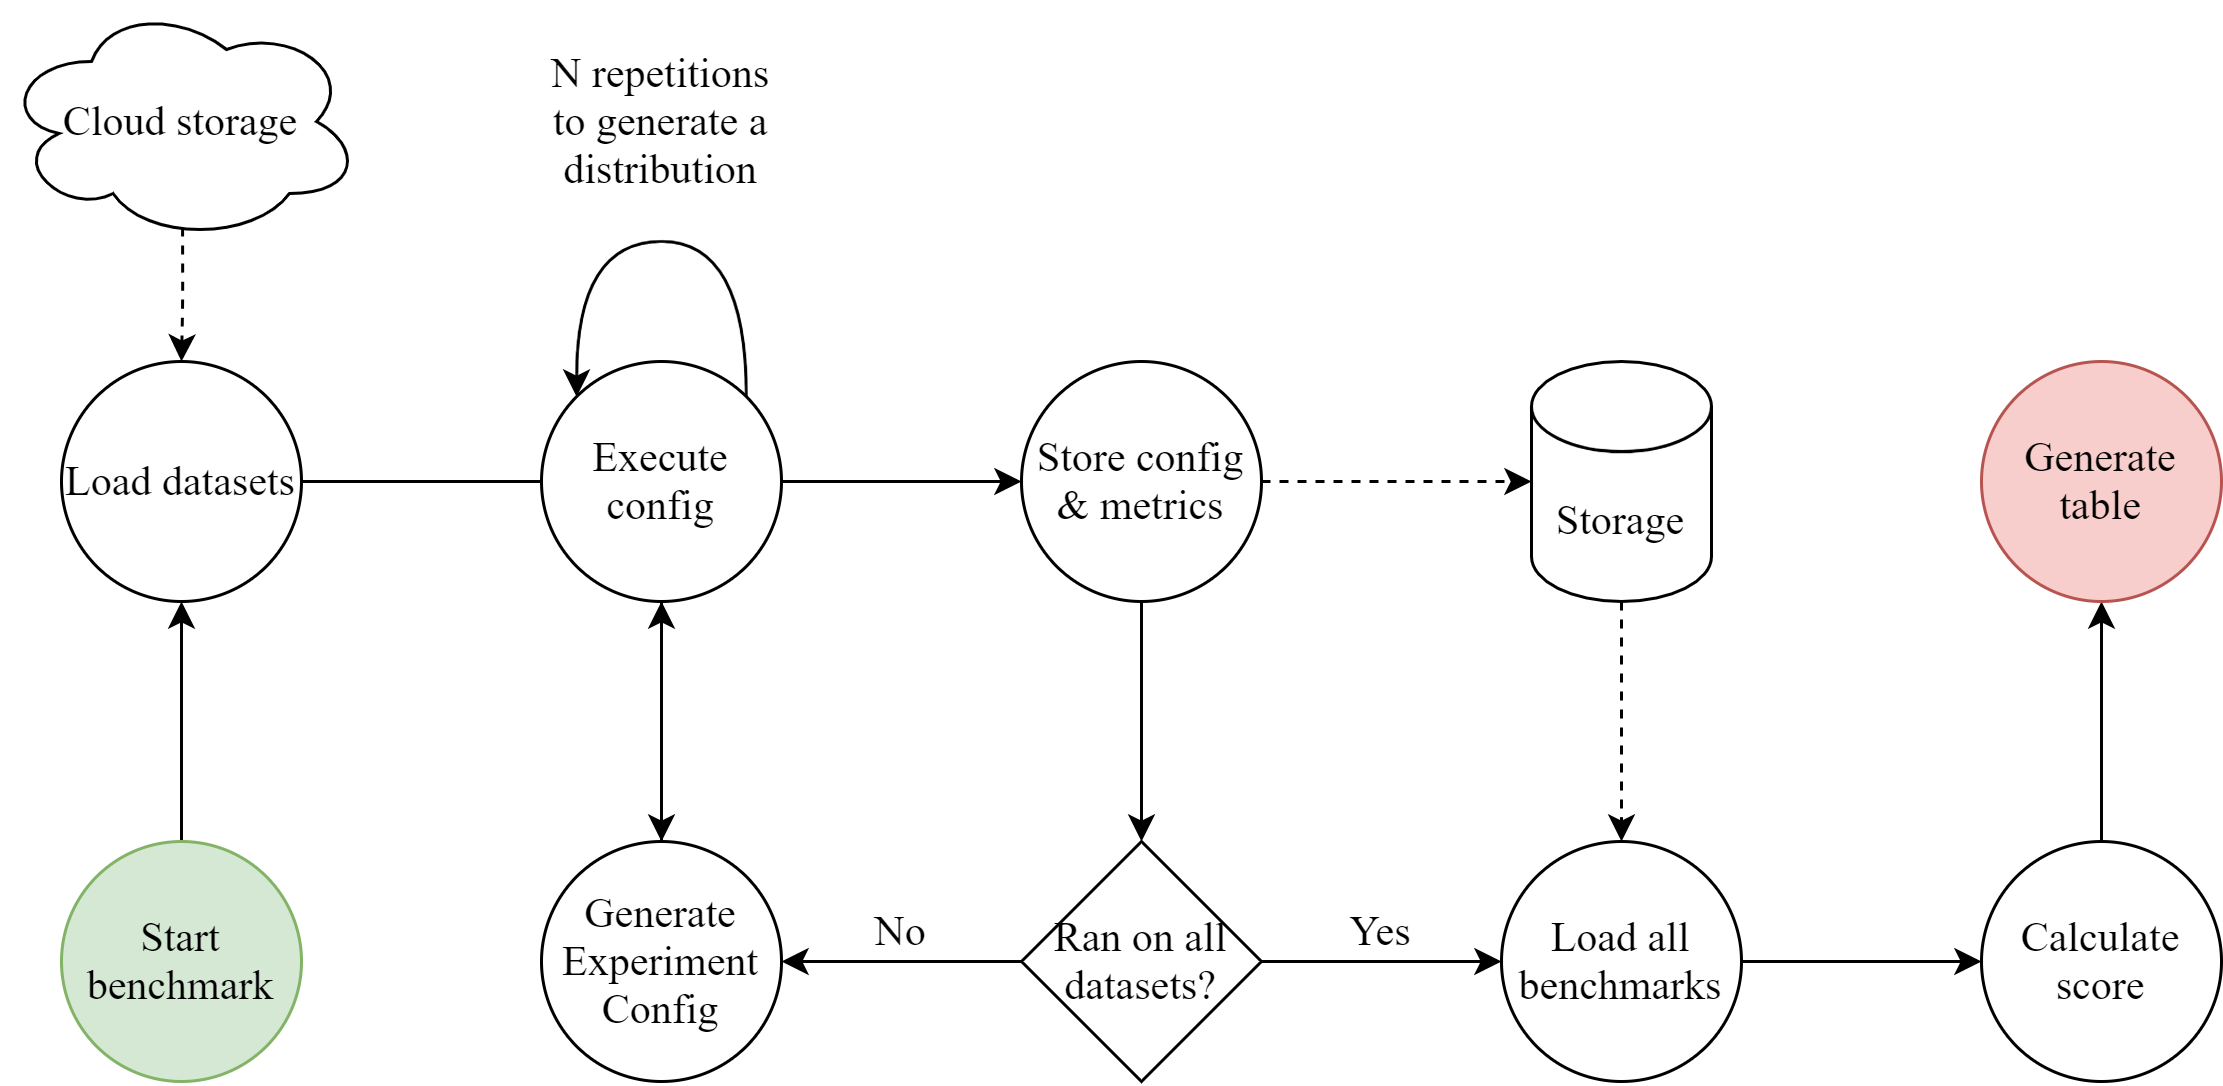
\includegraphics[width=\linewidth]{./img/benchmarking_system_architecture.png}
  \caption{Proposed benchmarking system.}
  \label{fig:proposed_benchmarking_system}
\end{figure}

The benchmarking loop is as follows: the algorithm configuration file is first loaded into the Runtool and an experiment is generated where the algorithm is executed on each of the datasets \textit{N} times. The value of \textit{N} is determined in Section \ref{sec:compairing_hypothesis_tests}. Each time the algorithm is executed, error metrics are reported by the Gluon-TS Backtesting functionality and these logs are captured by the Runtool and stored to a file or database for long term storage. This file will be referred to as the \textit{Benchmark Result File} (BRF) for the remainder of the thesis. Along with the distribution of error metrics, the config file used should be stored in the BRF to make it possible to rerun each benchmark.

The latest benchmarks error distribution is then aggregated through some scoring method which summarizes the distribution as a single value. This is then repeated for each previous benchmark which has been run. The resulting scores are then used to rank the algorithms against each other. A table is then presented to the user showing the relative rank of the latest benchmark compared to the previous benchmarks.

\section{Reproducing Benchmarks}
\label{sec:reproduce_benchmarks}
\begin{figure}[h]
  \centering
  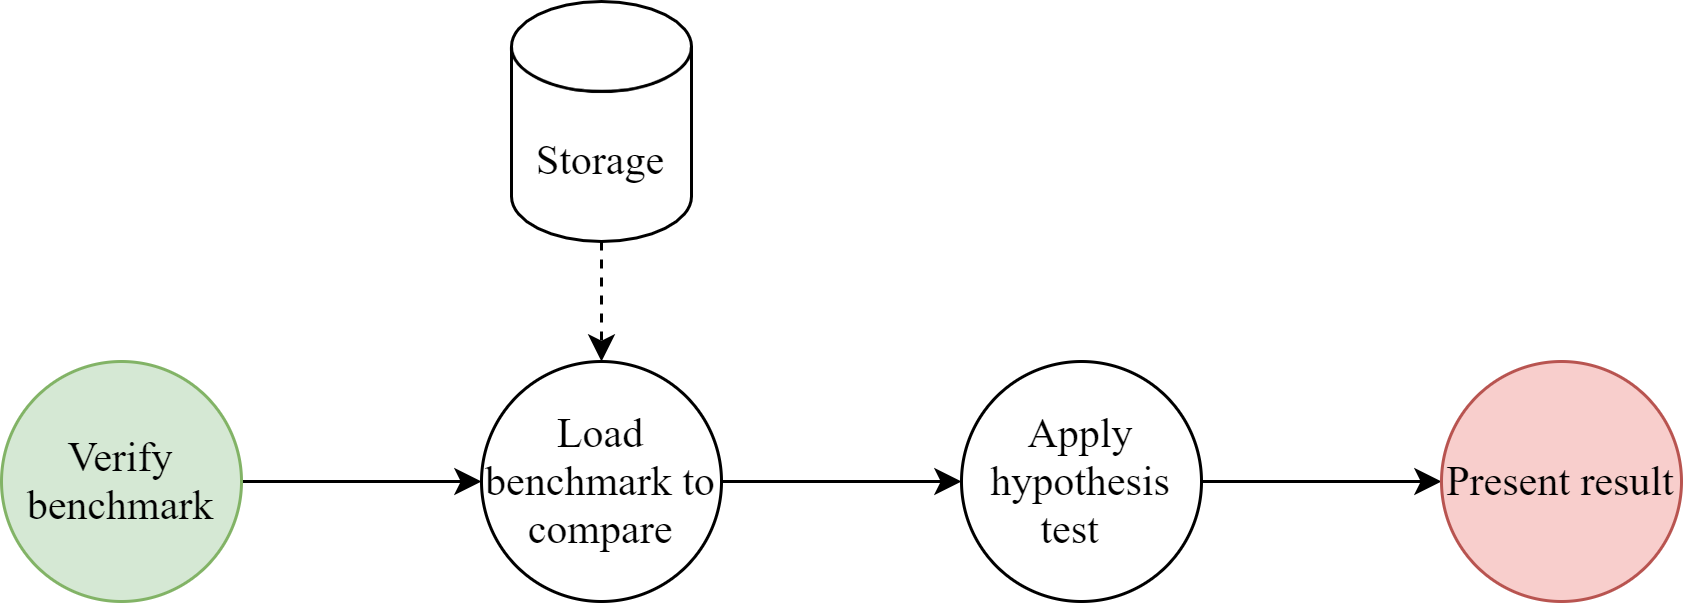
\includegraphics[width=\linewidth]{./img/verify_benchmark.png}
  \caption{Proposed system for verifying benchmarks.}
  \label{fig:proposed_validation_system}
\end{figure}
This section introduces a verification system which can assert statistical reproducibility to benchmarks, an overview over it can be seen in Figure \ref{fig:proposed_validation_system}.
In order to both technically and statistically be able to reproduce a benchmark, a user would need access to the image used and the BRF created by the benchmarking system. Provided these, the verification system could rerun the benchmark using the config file stored in the BRF and the provided image. Rerunning a benchmark with the same setup should result in a similar distribution being generated by the algorithm. Statistically speaking, if the algorithm in the image would be the same as the reference algorithm, both error metric distributions would be sampled from the same underlying distribution. The new distribution can then be compared with that of the benchmark stored in the BRF through a suitable hypothesis test.


\section{Hyperparameter Tuning}
\label{sec:hpo}
\begin{figure}[h]
  \centering
  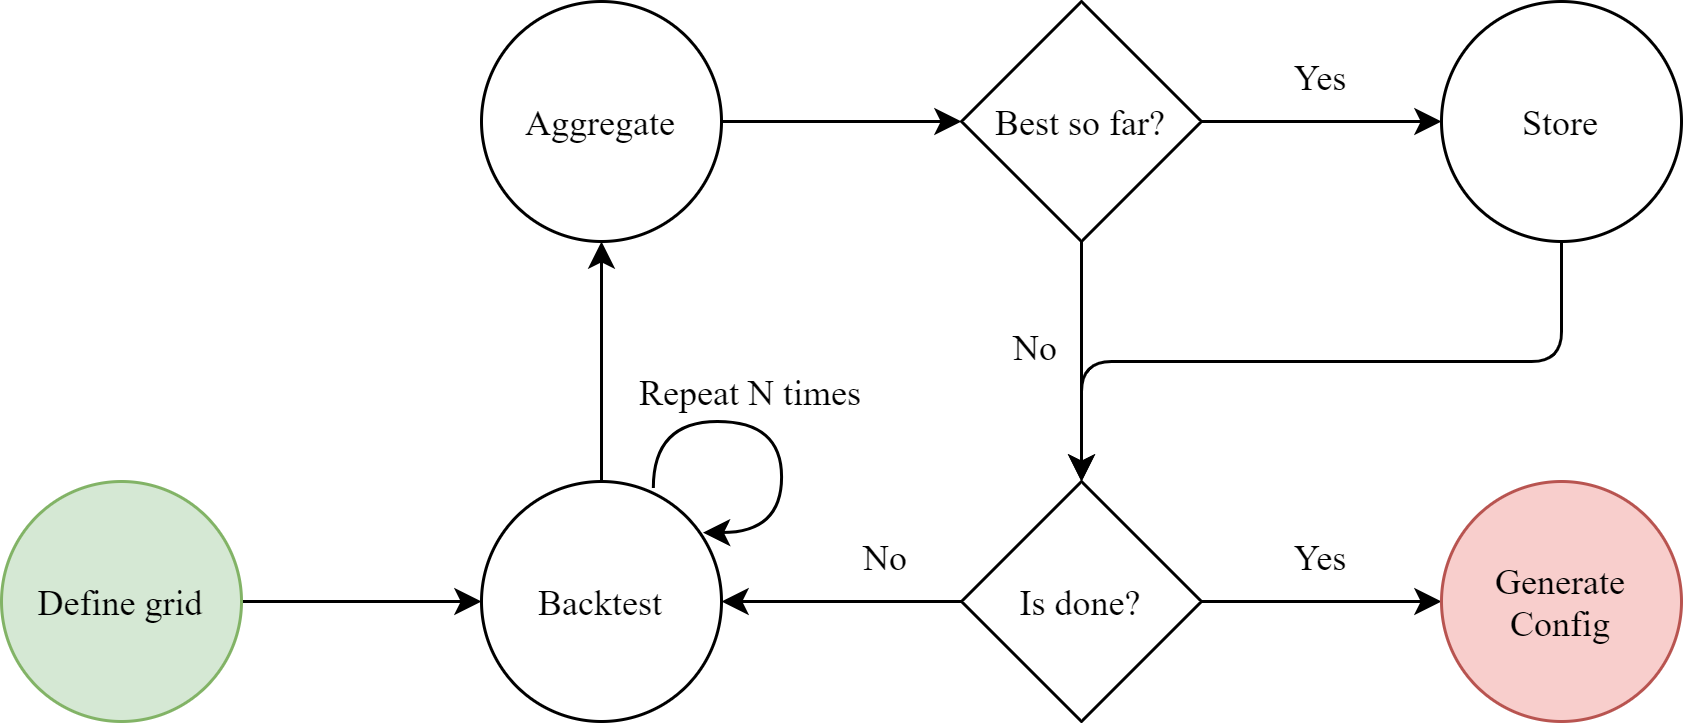
\includegraphics[width=\linewidth]{./img/tuning_overview.png}
  \caption{Proposed system for hyperparameter optimization with repeated runs.}
  \label{fig:proposed_hyperparameter_tuning}
\end{figure}
Hyperparameter tuning is a non-trivial task in itself and many advanced solutions exist such as Bayesian hyperparameter search, hyperband search or advanced meta learning approaches \cite{snoek2012practical,feurer2019hyperparameter, li2017hyperband}. The hyperparameter tuning approach proposed here is not intended to supersede these. Instead it focuses on taking the non deterministic output of each run into account when tuning. Figure \ref{fig:proposed_hyperparameter_tuning}, presents an overview of the proposed hyperparameter tuning system.

The proposed tuning system is in essence a simple grid search tuning algorithm with one major difference. Each configuration in the tuning loop is executed multiple times and then aggregated before being evaluated. Common ML frameworks which offer grid search such as SageMaker or SciKit-Learn (sklearn) surprisingly lack the capability to backtest each configuration multiple times \cite{sagemaker_website, scikit-learn}. While sklearn does offer a cross validation version of its grid search implementation, \textit{GridSearchCV}, this splits the dataset into multiple parts for each iteration. Thus it does not serve the same purpose as performing the backtest multiple times and aggregating the results.

Grid search was chosen as the tuning approach for this system as it is conceptually simple and it is a well known method. It does however have the downside that many unfavorable hyperparameter configurations are evaluated, something which e.g. bayesian search avoids \cite{snoek2012practical}.

An issue with the suggested tuning architecture is that time for tuning increases linearly with the number of repeated runs. Due to this, it may be suitable in real life scenarios to apply this approach as a second step after a set of promising hyperparameter configurations has been identified by another more time efficient approach.

\section{Dataset Analysis}
\label{sec:dataset_analysis}
It is common that new forecasting methods are compared on several datasets as to showcase their predictive power in different scenarios. Different datasets exhibit different characteristics such as trend and seasonality. By identifying a representable set of datasets with complementary characteristics, one can evaluate how robust a forecasting algorithm is to different datasets. Choosing a representable subset of datasets is also needed as the time to train an algorithm scales with the amount of datasets that it should be trained on. For an empirical comparison such as this, it is unfeasible to run training and tuning jobs for all algorithms and datasets available in Gluon-TS since this would take too long. In the remainder of this section an analysis of the datasets available in Gluon-TS is performed to identify a representable subset with diverse characteristics.

\subsection{Methodology}

For each dataset in Gluon-TS plots of the average time series along with one standard deviation from it is generated. This is done to get an overview of what the datasets looks like. Plotting time series for this purpose is common practice in time series forecasting, or as Hyndaman et al. so eloquently put in Forecasting: Principles and practice: \textit{"The first thing to do in any data analysis task is to plot the data."} \cite{hyndman_forecasting_3rd}.

\begin{figure}[htb]
  \centering
  \begin{subfigure}{0.49\textwidth}
    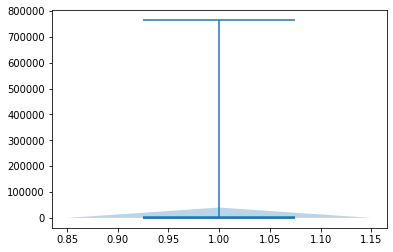
\includegraphics[width=\linewidth]{./img/electricity_violin_unscaled.png}
    \caption{Unscaled violin plot}
    \label{fig:electricity_violin_unscaled}
  \end{subfigure}
  \hfill
  \begin{subfigure}{0.49\textwidth}
    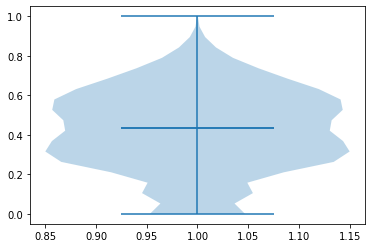
\includegraphics[width=\linewidth]{./img/electricity_violin.png}
    \caption{Scaled violin plot.}
    \label{fig:electricity_violin_scaled}
  \end{subfigure}
  \hfill
  \caption{Violin plots of the Electricity dataset with and without scaling.}
\end{figure}

% \begin{figure}[htb]
%   \centering
%   \minipage{0.5\textwidth}
%   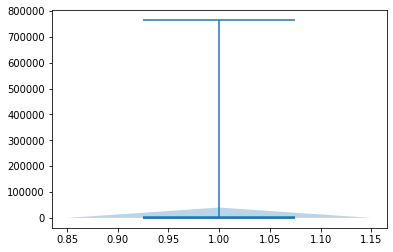
\includegraphics[width=\linewidth]{./img/electricity_violin_unscaled.png}
%   \caption{Unscaled violin plot}
%   \label{fig:electricity_violin_unscaled}
%   \endminipage\hfill
%   \minipage{0.5\textwidth}
%   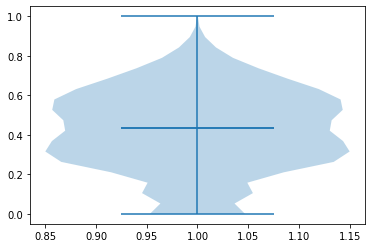
\includegraphics[width=\linewidth]{./img/electricity_violin.png}
%   \caption{Scaled violin plot}
%   \label{fig:electricity_violin_scaled}
%   \endminipage\hfill
%   \caption{Violin plots of the Electricity dataset with and without scaling.}
% \end{figure}

A common tool for visualising time series is to generate a histogram of the time series data. However as the datasets available in Gluon-TS contains tens of thousands of time series, plotting each of these individually is unfeasible. Instead the average time series and one standard deviation of its values is plotted. Another common method for visualizing single time series is to generate a histogram of its values \cite{hyndman_forecasting_3rd}. Instead of generating such histograms violin plots are used in as these capture both the distribution of values just as histograms do as well as the median value and the interquartile range. Since each time series is on its own scale, the aggregate violin plots are hard to read as seen in Figure \ref{fig:electricity_violin_unscaled}. By scaling each time series in the dataset by the maximum value of that time series before plotting it the violin plot becomes easier to interpret, see Figure \ref{fig:electricity_violin_scaled}.

In addition to the visual tools the following statistics is calculated for each of the datasets in Gluon-TS:

\begin{itemize}
  \item Mean value
  \item Max value
  \item Min value
  \item Number of time series
  \item Number of datapoints
  \item Length of shortest time series
  \item Length of longest time series
  \item Strength of the trend (mean and standard deviation)
  \item Strength of the seasonality (mean and standard deviation)
\end{itemize}

Simple metrics such as the maximum, mean and minimum values provide a high level overview of the dataset and helps identifying possible issues which can surface further down the line. For example, the MAPE metric is unstable for time series close to zero as a division with zero occurs \cite{goodwin_asymmetry_1999}.

The number of time series are important for global models as these then have more data which they can learn across which help to combat overfitting. However, the number of time series is not important for local models as these are only impacted by the quality and length of each individual time series. Longer time series however, benefit forecasting models which can handle longer horizons \cite{makridakis_m4_2020}.

For these reasons, the number of time series and the lengths of the shortest and longest time series are necessary metrics when comparing datasets. Optimally one would have both long time series and many series as this would benefit both global and local models.

K-fold cross validation as discussed in Section \ref{sec:evaluating_performance} is a method for increasing the number of series in a dataset. Most of the datasets in Gluon-TS have had K-fold cross validation applied to them already. Thus the potential size after applying K-fold cross validation should be considered for those datasets for which it has not yet been applied.

In Chapter \ref{cha:chapter2}, it was shown that the strength of seasonality (SoS) and the strength of the trend (SoT) of time series are useful metrics for differentiating time series. Due to this, these two measures are the main criterias by which the datasets are chosen. Since each dataset can have both a SoT and SoS, the most diverse datasets are those with complimentary SoT and SoS. In total four datasets can then be identified which fullfill these criteria; one with both high SoT and high SoS, one with high SoT and low SoS, one with low SoT and high SoS and one with both low SoT and low SoS. Since each time series within a dataset is unlikely to have the same SoT or SoS also the variance of the SoT and SoS need to be taken into account. Thus, when two datasets have similar strength, the one with the lowest variance is chosen. This emphasizes the diversity of the datasets as two datasets with high variance in SoS or SoT are prone to contain more similar time series having similar SoT and SoS.

Since larger datasets make models less prone to overfit, the largest dataset is chosen in case of a tie where two datasets are exhibiting a negligible difference in SoT and SoA. Table \ref{dataset_criteria} presents the criterias used for identifying a representable subset of datasets.

\begin{table}[h]
  \begin{tabular}{cc}
    \# & Criteria                                         \\
    1  & One dataset with high trend and low seasonality  \\
    2  & One dataset with low trend and high seasonality  \\
    3  & One dataset with low trend and low seasonality   \\
    4  & One dataset with high trend and high seasonality \\
    5  & Lower variance of strengths is prefered          \\
    6  & Larger dataset chosen in case of a tie           \\
  \end{tabular}
  \caption{Criteria for identifying a representable subset of datasets.}
  \label{dataset_criteria}
\end{table}


\subsubsection{Limitations}
The M4 dataset does not significantly differ to the M3 dataset except for its size \cite{m3_vs_M4}. Thus, the M3 dataset is not considered in this comparison. Another set of datasets which are not going to be used are the NIPS datasets. This is due to them having had postprocessing applied to them. As the exact post processing is not known, comparing any findings when training on these datasets with other papers becomes hard and introduces uncertainty.

\subsection{Result}
To calculate the strengths of the trend and seasonality, a STL decomposition is needed for each time series in the dataset. This decomposition is done using the STL method of the Statsmodel package in Python \cite{seabold2010statsmodels}. The SoS is then calculated using Equation \ref{eq:strength_of_seasonality} and the SoT is calculated using Equation \ref{eq:strength_of_trend}. To summarize the strengths, the mean value and the standard deviation is then calculated of the SoS \& SoT for each dataset.

The complete plots and statistics are available in the appendix as they were to numerous to be displayed here. However a summary of the extracted statistics is presented in Table \ref{tab:dataset_statistics}.


\begin{table}[h]
  \pgfplotstabletypeset[
    color cells={min=0,max=1},
    col sep=comma,
    columns/Dataset/.style={reset styles,string type},
    /pgfplots/colormap={whiteblue}{rgb255(0cm)=(255,255,255); rgb255(1cm)=(2,138,4)},
    /pgf/number format/.cd,
    fixed,
    fixed zerofill,
    precision=2,
  ]{
    Dataset,Trend,Seasonality,Trend Dev., Seasonality Dev.
    Exchange Rate,1,0.12,0,0.3
    M4 Daily, 0.98,0.05,0.05,0.1
    M4 Yearly,0.93,0.09,0.13,0.16
    M4 Quarterly,0.9,0.2,0.16,0.27
    M4 Monthly, 0.84,0.32,0.32,0.3
    M4 Weekly,0.77,0.31,0.31,0.35
    Electricity,0.65,0.84,0.17,0.19
    M4 Hourly,0.62,0.88,0.37,0.16
    Wiki Rolling, 0.53,0.23,0.27,0.26
    M5,0.38,0.28,0.32,0.33
    Traffic,0.16,0.67,0.12,0.1
    Solar Energy, 0.09,0.84,0.03,0.02
    Taxi,0.02,0.66,0.02,0.08
  }
  \caption{Strength of trend \& seasonality for datasets in Gluon-TS.}
  \label{heatmap_strengths}
\end{table}

There is only one dataset in Table \ref{heatmap_strengths} which exhibits low trend and low seasonality and that is the M5 dataset. However the M5 dataset does show the most variance of all the datasets which implies that it contains many time series with and without trend and seasonality. Despite this, since it is the largest dataset available and that there are no other datasets which exhibit low average trend \& seasonality, the M5 dataset is deemed appropriate for use in the benchmarking system.

\clearpage
\begin{table}[htb]
  \begin{tabular}{c | c c c c c c c c c}
    \rothalf{Dataset} & \rothalf{Mean} & \rothalf{Series} & \rothalf{Items} & \rothalf{Shortest} & \rothalf{Longest} & \rothalf{Min} & \rothalf{Max} & \rothalf{Freq.} \\ [0.5ex]
    \hline
    Elec.             & 2510.68        & 321              & 6755124         & 21044              & 21044             & 0.0           & 764000.0      & 1H              \\
    Elec.             & 2509.92        & 2247             & 47501580        & 21068              & 21212             & 0.0           & 764000.0      & 1H              \\
    \hline
    Exch.             & 0.68           & 8                & 48568           & 6071               & 6071              & 0.01          & 2.11          & 1B              \\
    Exch.             & 0.68           & 40               & 246440          & 6101               & 6221              & 0.01          & 2.11          & 1B              \\
    \hline
    Solar             & 40.35          & 137              & 960233          & 7009               & 7009              & 0.0           & 509.05        & 10min           \\
    Solar             & 40.25          & 959              & 6813695         & 7033               & 7177              & 0.0           & 509.05        & 10min           \\
    \hline
    Traf.             & 0.06           & 862              & 12099032        & 14036              & 14036             & 0.0           & 0.72          & H               \\
    Traf.             & 0.06           & 6034             & 85272488        & 14060              & 14204             & 0.0           & 0.72          & H               \\
    \hline
    Exch.*            & 0.68           & 8                & 48568           & 6071               & 6071              & 0.01          & 2.11          & B               \\
    Exch.*            & 0.68           & 40               & 246440          & 6101               & 6221              & 0.01          & 2.11          & B               \\
    \hline
    Elec.*            & 607.95         & 370              & 2142282         & 1081               & 5833              & 0.0           & 168100.0      & H               \\
    Elec.*            & 652.36         & 2590             & 10340239        & 1105               & 4000              & 0.0           & 168100.0      & H               \\
    \hline
    Solar*            & 40.35          & 137              & 960233          & 7009               & 7009              & 0.00          & 509.05        & H               \\
    Solar*            & 40.25          & 959              & 6813695         & 7033               & 7177              & 0.00          & 509.05        & H               \\
    \hline
    Traf.*            & 0.05           & 963              & 3852963         & 4001               & 4001              & 0.00          & 1.00          & H               \\
    Traf.*            & 0.05           & 6741             & 26964000        & 4000               & 4000              & 0.00          & 1.00          & H               \\
    \hline
    Wiki              & 3720.54        & 9535             & 7551720         & 792                & 792               & 0.00          & 7752515.00    & D               \\
    Wiki              & 3663.55        & 47675            & 40619100        & 792                & 912               & 0.00          & 7752515.00    & D               \\
    \hline
    Taxi              & 8.79           & 1214             & 1806432         & 1488               & 1488              & 0.0           & 265.0         & 30min           \\
    Taxi              & 7.41           & 67984            & 54999056        & 149                & 1469              & 0.0           & 225.0         & 30min           \\
    % \hline
    % M3 Mo.            & 4928.47        & 1428             & 141858          & 48                 & 126               & 80.00         & 86730.00      & M                   \\
    % M3 Mo.            & 4971.28        & 1428             & 167562          & 66                 & 144               & -1200.00      & 86730.00      & M                   \\
    % \hline
    % M3 Q              & 4819.27        & 756              & 30956           & 16                 & 64                & 126.00        & 20245.00      & 3M                  \\
    % M3 Q              & 4983.53        & 756              & 37004           & 24                 & 72                & 121.00        & 20375.00      & 3M                  \\
    % \hline
    % M3 Y              & 4417.05        & 645              & 14449           & 14                 & 41                & 30.00         & 39666.22      & 12M                 \\
    % M3 Y              & 4815.77        & 645              & 18319           & 20                 & 47                & 30.00         & 45525.66      & 12M                 \\
    % \hline
    % M3 O              & 6152.18        & 174              & 11933           & 63                 & 96                & 28.00         & 59472.00                            \\
    % M3 O              & 5999.87        & 174              & 13325           & 71                 & 104               & 28.00         & 59472.00                            \\
    \hline
    M4 H              & 6827.69        & 414              & 353500          & 700                & 960               & 10.00         & 703008.00     & H               \\
    M4 H              & 6859.56        & 414              & 373372          & 748                & 1008              & 10.00         & 703008.00     & H               \\
    \hline
    M4 D              & 4951.40        & 4227             & 9964658         & 93                 & 9919              & 15.00         & 352000.00     & D               \\
    M4 D              & 4960.15        & 4227             & 10023836        & 107                & 9933              & 15.00         & 352000.00     & D               \\
    \hline
    M4 W              & 3738.52        & 359              & 366912          & 80                 & 2597              & 104.69        & 51410.00      & W               \\
    M4 W              & 3755.97        & 359              & 371579          & 93                 & 2610              & 104.69        & 51410.00      & W               \\
    \hline
    M4 M              & 4193.28        & 48000            & 10382411        & 42                 & 2794              & 20.00         & 132731.31     & M               \\
    M4 M              & 4207.51        & 48000            & 11246411        & 60                 & 2812              & 20.00         & 177950.00     & M               \\
    \hline
    M4 Q              & 4141.00        & 24000            & 2214108         & 16                 & 866               & 19.50         & 82210.70      & 3M              \\
    M4 Q              & 4287.13        & 24000            & 2406108         & 24                 & 874               & 19.50         & 82210.70      & 3M              \\
    \hline
    M4 Y              & 3630.52        & 23000            & 715065          & 13                 & 300               & 22.10         & 115642.00     & 12M             \\
    M4 Y              & 4076.24        & 23000            & 852909          & 19                 & 300               & 22.00         & 158430.00     & 12M             \\
    \hline
    M5                & 1.12           & 30490            & 57473650        & 1885               & 1885              & 0.00          & 763.00        & D               \\
    M5                & 1.13           & 30490            & 58327370        & 1913               & 1913              & 0.00          & 763.00        & D               \\
    \hline
  \end{tabular}
  \caption{Statistics of the datasets, top row for each dataset is the train split, the bottom row is the test split.}
  \label{tab:dataset_statistics}
\end{table}
\clearpage

In order to choose a dataset which fits into the category of high seasonality and low trend there are three options; Solar Energy, Taxi and Traffic. Of these the Solar Energy dataset has the lowest variance for both the trend and the seasonality. This in addition to having the second lowest average trend of the three and \(23\)\% higher average seasonality than the Taxi and the Traffic datasets makes it most suitable according to the criteria in Table \ref{dataset_criteria}.

The datasets with the lowest seasonality and the highest trends are the M4 datasets except for the M4 Hourly as well as the Exchange rate dataset. The one with the lowest variance and the highest trend of these is the Exchange Rate dataset closely followed by the M4 Daily dataset. The M4 Daily has lower variance for both strength and seasonality, and Table \ref{tab:dataset_statistics} shows that the size of the Exchange Rate dataset is only 8 time series and 48k datapoints in comparison to the 4227 series and 9.9M datapoints the M4 Daily dataset. Thus the M4 Daily is more suited than the Exchange Rate dataset as a representable dataset. Furthermore, all other M4 datasets exhibit a higher variance than the M4 Daily which enforces the M4 Daily to be a better choice for this comparison.

When it comes to finding a dataset which exhibit both high trend and a high seasonality, there are only two options, the Electricity dataset and the M4 Hourly dataset. They both have a high variance, however the variance of the Electricity dataset is slightly lower than that of M4 Hourly. In addition, the Electricity dataset has almost twice the amount of datapoints as M4 Hourly. Thus the Electricity dataset is chosen as it fits the criteria better.

% \begin{figure}[htb]
%   \centering
%   \minipage{0.48\textwidth}
%   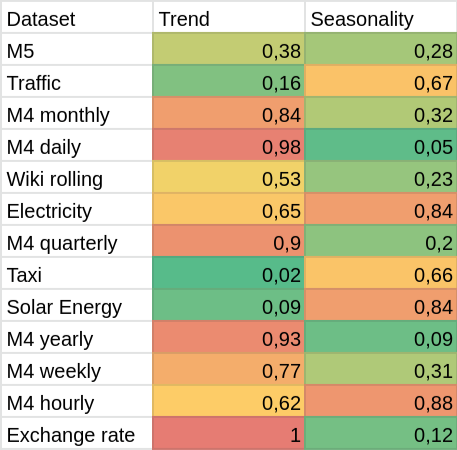
\includegraphics[width=\linewidth]{./img/dataset_trend_seasonality_heatmap_mean.png}
%   \caption{Heatmap of the strength of the trend and the seasonality sorted by the size of the datasets.}
%   \endminipage\hfill
%   \minipage{0.48\textwidth}
%   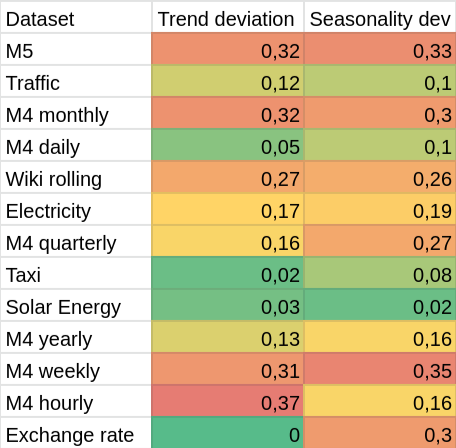
\includegraphics[width=\linewidth]{./img/dataset_trend_seasonality_heatmap_deviation.png}
%   \caption{Heatmap of the standard deviation of the strength of the trend and the seasonality for the datasets.}
%   \endminipage\hfill
% \end{figure}  

To summarize the four datasets which most closely fit the criteria from Table \ref{dataset_criteria} are:

\begin{table}[htp]
  \centering
  \begin{tabular}{ccc}
                              & \textbf{Low trend} & \textbf{High Trend} \\
    \hline
    \textbf{Low seasonality}  & M5                 & M4 Daily            \\
    \hline
    \textbf{High Seasonality} & Solar Energy       & Electricity         \\
  \end{tabular}
  \caption{Datasets with complimentary strengths of trend and seasonality}
  \label{fig:representative_subset_of_datasets}
\end{table}

\section{Comparing Tests for Validating Forecasting Performance}
\label{sec:compairing_hypothesis_tests}
This section investigates the performance of three hypothesis tests for use on distributions of error metrics. The investigated tests are the T-test, Welch’s T-Test and the Kolmogorov-Smirnov two sample test.

Gluon-TS catches accuracy regressions through checking whether new forecasts are within \(1.645\) standard deviations, i.e., within the 95th percentile of past values \cite{gluonts-github}. This approach is based on the assumption that the distribution of error metrics is normally distributed. If this is true then, this simpler approach may be more suitable than a hypothesis test for reproducibility. Thus this approach will be evaluated along with the hypothesis tests.

In order to decide which tests are suitable, certain aspects of the tests and the data need to be investigated. Since the naive test and the parametric tests rely on that the distributions are well defined to function it is important to identify how error distributions of forecasting methods look like, i.e., is it normally distributed or do they follow other distributions.

Different tests require different amount of samples to be accurate, and some tests can become unstable if the sample sizes differ too much \cite{hassani2015kolmogorov, student_or_welch}. Since performing a benchmark is time consuming, it is beneficial from a time perspective to collect as few samples as possible. Thus identifying how the tests perform when applied to different sample sizes is important as a minimum sample size can be identified.

A summary of the questions this minor study aim to answer are:

\begin{itemize}
  \item Which test is best for limited data
  \item Is a parametric test suitable or is a non-parametric test needed
  \item What is a reasonable sample size
  \item Which test has the lowest false reject ratio for related distributions
  \item Is a naive standard deviation based test sufficient
\end{itemize}


\subsection{Methodology}
\label{hypothesis_test_methodology}
Several of the questions which need to be answered require distributions of error metrics to be collected. For this purpose, the DeepAREstimator presented in Section \ref{algo:deepar} is suitable as it is both quick to train and a non-trivial forecaster. The dataset chosen is the Electricity dataset since it is a medium to small sized dataset, thus shortening the required training time.

The Runtool is then used to create 900 experiments where the DeepAREstimator is executed on the Electricity dataset. 300 of these runs has the hyperparameter \textit{distr\_output} set to StudentTOutput, 300 runs are executed with \textit{distr\_output} set to use the NegativeBinomialDistribution. The remaining 300 runs are executed using the Poisson distribution. The three distributions generated by these 900 training jobs are referred to as NB, ST and P in this chapter.

After the distributions are collected, histograms of the distributions are created to identify whether the distributions are visually different. This is done since if all three are visually similar it is unlikely that they can be used for evaluating the hypothesis tests. Further, a visual analysis can determine whether the naive method and or the T-test is suitable since it requires normally distributed data.

After the visual analysis, the ratio of false rejects are calculated, i.e., how often the test is unable to detect that two samples are sampled from the same distribution. To answer this questions, let \(N\) be the total distribution and \(X,Y\) be the two samples drawn from \(N\). The size of \(X\) is then defined by \[k \leq |X| \leq |N| - |Y|\] where \(k\) is a constant value. Similarly, the size of \(Y\) varies between: \[k	\leq |Y| \leq |N|-k\] For each sample of \(X\) and \(Y\) the tests are applied and false negatives are recorded.

In order to evaluate a suitable minimum sample size, heatmaps are generated where the tests are applied to the three distributions with varying sample sizes. Each test is performed with a \textit{P value} of 0.05. If the test accepts the samples to be from the same distribution the color green is used while a rejection, is colored red.

\subsection{Results}

\begin{figure}[htb]
  \centering
  \minipage{0.49\textwidth}
  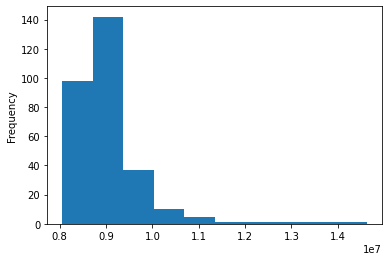
\includegraphics[width=\linewidth]{./img/histogram_deepar_electricity_statistics_300_samples.png}
  \caption{Student-T}
  \label{deepar_student_t_distibution}
  \endminipage\hfill
  \minipage{0.49\textwidth}
  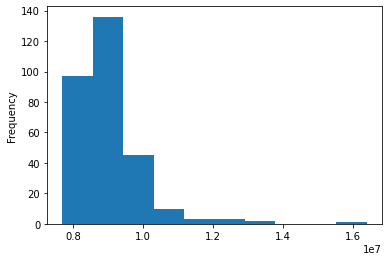
\includegraphics[width=\linewidth]{./img/histogram_deepar_negbin_electricity_statistics_200_samples.png}
  \caption{Neg-Binomial}
  \label{deepar_negbinomial_distibution}
  \endminipage\hfill
  \\
  \minipage{0.49\textwidth}
  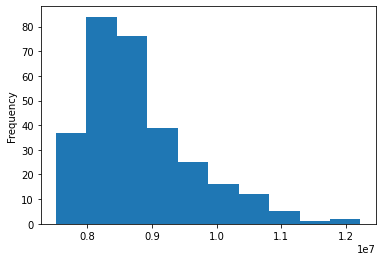
\includegraphics[width=\linewidth]{./img/histogram_deepar_poisson_electricity_statistics_200_samples.png}
  \caption{Poisson}
  \label{deepar_poisson_distribution}
  \endminipage
  \caption{Histograms of the absolute error for 300 runs of DeepAR on the Electricity dataset with three different values of the hyperparameter \emph{distr\_output}}
  \label{deepar_elec_300_hist}
\end{figure}


The histograms shown in Figure \ref{deepar_elec_300_hist} do not resemble a normal distribution. Instead all three histograms are more closely approximating a log normal distribution. Note that the histogram in Figure \ref{deepar_student_t_distibution} and \ref{deepar_negbinomial_distibution} are very similar while the one in Figure \ref{deepar_elec_300_hist} differs. This indicates that different hyperparameter configurations for a single algorithm impacts the error distribution.


\begin{table}[htp]
  \centering
  \begin{tabular}{lcccc}
    {\textbf Name}    & {\textbf \%} & {\textbf configuration} \\
    \hline
    Naive             & $<$1\%       & Negative Binomial       \\
    Naive             & $<$1\%       & Student T               \\
    Naive             & $<$1\%       & Poisson                 \\
    \hline
    T-Test            & 5\%          & Negative Binomial       \\
    T-Test            & 5\%          & Student T               \\
    T-Test            & 32\%         & Poisson                 \\
    \hline
    Welchs T-Test     & 11\%         & Negative Binomial       \\
    Welchs T-Test     & 8\%          & Student T               \\
    Welchs T-Test     & 31\%         & Poisson                 \\
    \hline
    Kolmogorv-Smirnov & 3\%          & Negative Binomial       \\
    Kolmogorv-Smirnov & 5\%          & Student T               \\
    Kolmogorv-Smirnov & 21\%         & Poisson                 \\
    \hline
  \end{tabular}
  \caption{Number of times when the algorithm failed to recognize that the samples were from the same distribution}
  \label{tab:false_rejects}
\end{table}

In Table \ref{tab:false_rejects} the amount of false rejections of the three hypothesis tests and the naive solution is presented. From this data it is clear that the Naive solution is the best performing with a 1\% chance of failing to validate that the two samples are from the same distribution. The Kolmogorov-Smirnov performs second best, however it is incorrect 21\% of the time when evaluating on the distribution generated by the Poisson configuration. The two T-Tests are the worst performers, performing worse than or equal to the Kolmogorov-Smirnov test on all distributions.

Since the distributions of error metrics are not reminiscent of the normal distribution, the naive method, the T-test and the Welch's T-test which are parametric tests are unsuitable for use when verifying dataset distributions. The data in Table \ref{tab:false_rejects} further enforces this since Kolmogorov-Smirnov is the second best performer for all distributions where only the naive method is better. In Figure \ref{naive_negative_bin_poisson} the naive method is evaluated on the Poisson and Negative Binomial distributions. It is clear from this heatmap that the naive method is prone to accept quite different distributions for all but small sample sizes. This behaviour is also apparent on all other heatmaps where the naive method is used, see Appendix \ref{app:naive_heatmaps}. This is expected since the distributions all have similar average values even though their distributions are visually different. In comparison, the Kolmogorov-Smirnov test is able to differentiate all distributions given sufficient sample sizes, see Figures \ref{ks_student_t_poisson}, \ref{ks_student_t_neg_bin}, \ref{ks_neg_bin_poisson}.

The sample size required to differentiate between different distributions (true negatives) as well as the sample sizes required for true positives for the Kolmogorov-Smirnov test is presented in Table \ref{tab:required_sample_sizes}. This table summarizes the heatmaps generated for the Kolmogorov-Smirnov test when applied to samples of varying sizes from the three distributions as described in \ref{hypothesis_test_methodology}. Additional heatmaps not shown in this chapter are available in Appendix \ref{app:heatmaps}.


\begin{table}[htp]
  \centering
  \begin{tabular}{cccc}
                      & Student T & Poisson & Negative Binomial \\
    \hline
    Student T         & \(>50\)   &         &                   \\
    \hline
    Poisson           & \(>25\)   & \(>45\) &                   \\
    \hline
    Negative Binomial & \(>160\)  & \(>60\) & \(<130\)          \\
  \end{tabular}
  \caption{Required sample sizes for the Kolmogorov Smirnov test on three distributions of error metrics.}
  \label{tab:required_sample_sizes}
\end{table}

\begin{figure}[h]
  \centering
  \minipage{0.7\textwidth}
  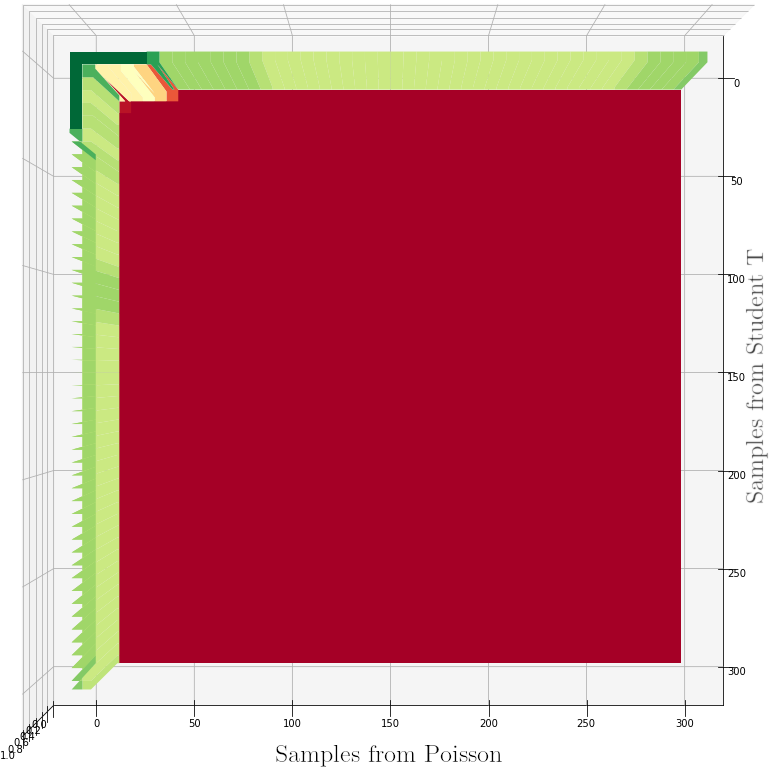
\includegraphics[width=\linewidth]{./img/hypothesis_test/deepar_heatmap_Y_student_t_X_poisson_ks_edited.png}
  \endminipage
  \caption{Heatmap of KS applied to the ST and P distributions.}
  \label{ks_student_t_poisson}
\end{figure}
\clearpage

From Table \ref{tab:required_sample_sizes} it is shown that the KS test becomes accurate for true positives at a sample size of at least 40 samples. However, it seems as if KS can become unstable for sample sizes above 130. To be able to use the KS statistic to distinguish between different distributions, sample sizes above 160 may be needed if the distributions are visually very similar, otherwise, sample sizes above \(60\) suffice. These values are aligned with the findings of the simulation study performed by Hassani et al. \cite{hassani2015kolmogorov}. There they showed the need for \(>128\) samples to achieve \(>99\)\% rejection rate for similarly looking distributions.

\begin{figure}[h]
  \centering
  \minipage{0.7\textwidth}
  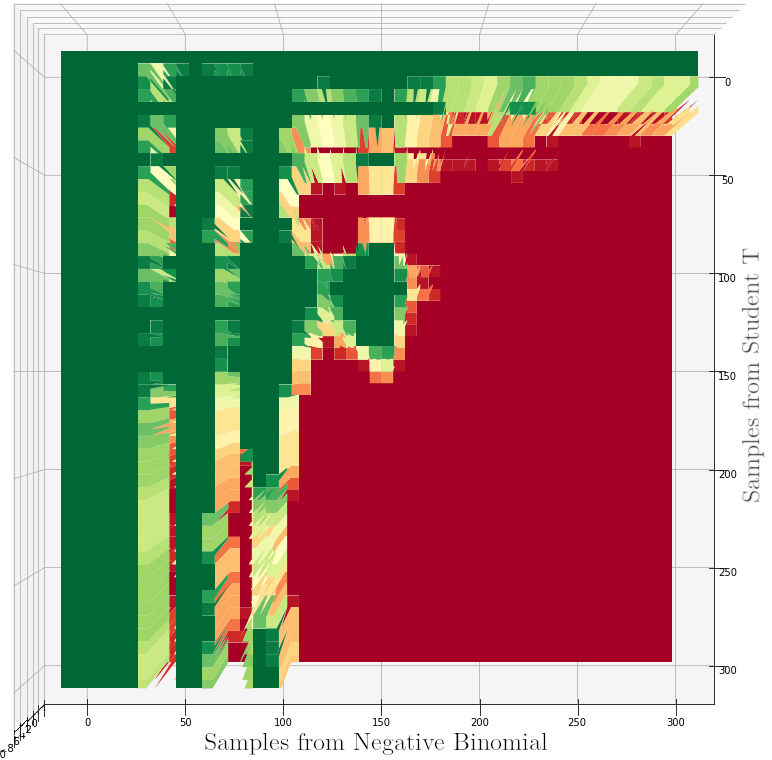
\includegraphics[width=\linewidth]{./img/hypothesis_test/deepar_heatmap_Y_student_t_X_neg_bin_ks_edited.png}
  \caption{Heatmap of KS applied to the ST and NB distributions.}
  \label{ks_student_t_neg_bin}
  \endminipage
\end{figure}

To summarize, despite the limited data available for this comparison, the Naive test, the T-test and Welch’s T-Test has been shown to be unsuitable for comparing distributions of time series forecasting errors due to non-normality of the data. This makes the Kolmogorov-Smirnov two sample test the best suited statistical test for asserting the statistical reproducibility of error metric distributions. When evaluating the Kolmogorov-Smirnov on samples from three different distributions it was shown that \(>60\) samples are required to verify distributions but more than \(160\) may be required to differentiate similar distributions.

\begin{figure}[h]
  \centering
  \minipage{0.65\textwidth}
  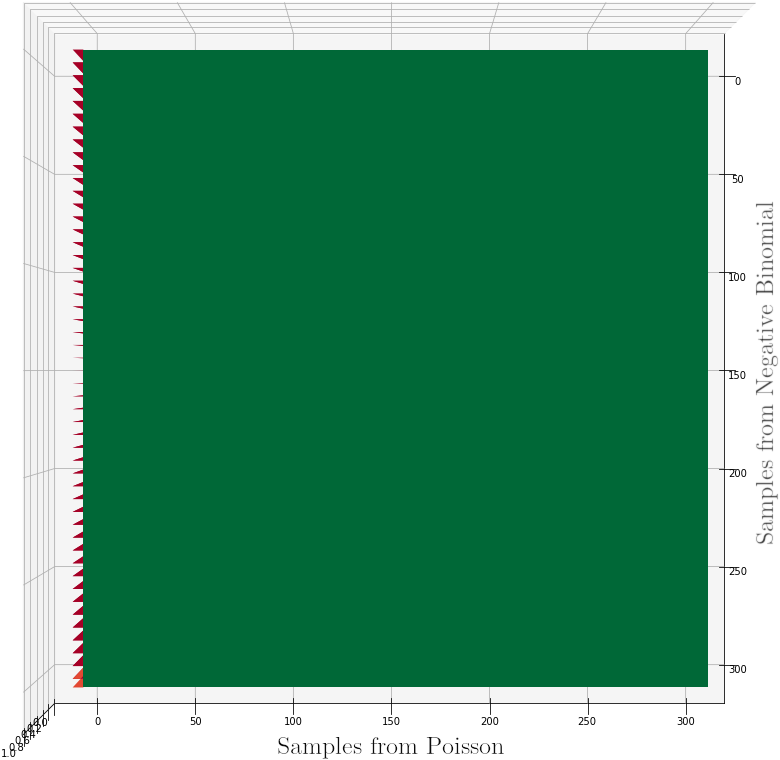
\includegraphics[width=\linewidth]{./img/hypothesis_test/deepar_X_poisson_Y_neg_bin_naive_edited.png}
  \caption{Heatmap of the Naive method applied to the NB and P distributions.}
  \label{naive_negative_bin_poisson}
  \endminipage
  \\
  \minipage{0.65\textwidth}
  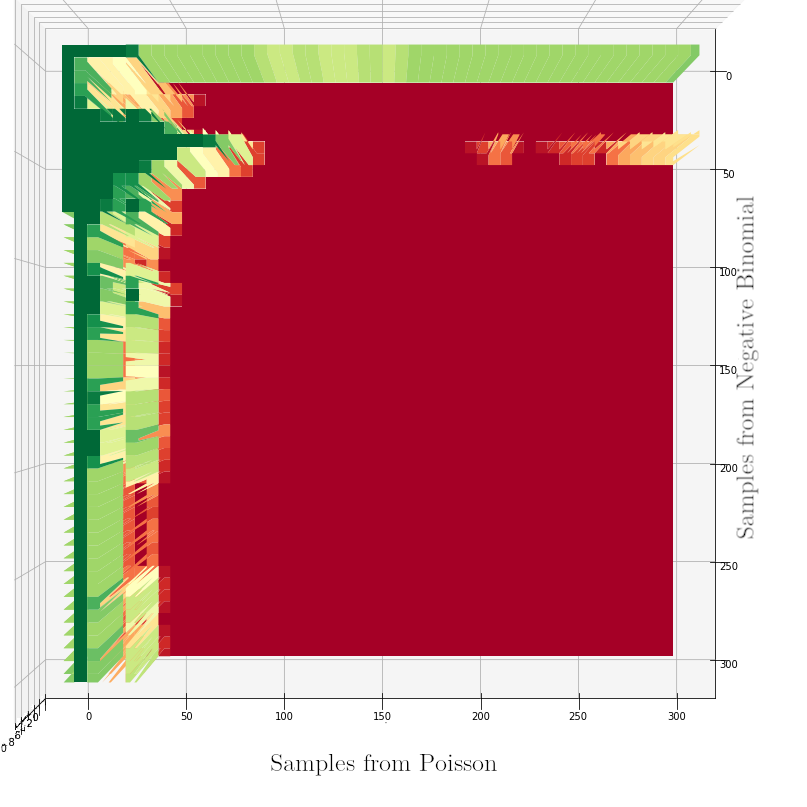
\includegraphics[width=\linewidth]{./img/hypothesis_test/deepar_heatmap_Y_neg_bin_X_poisson_ks_edited_labels.png}
  \caption{Heatmap of KS applied to the NB and P distributions.}
  \label{ks_neg_bin_poisson}
  \endminipage
\end{figure}
\clearpage

\section{Ranking Distributions}
\label{sec:ranking_distributions}
To rank algorithms based on distributions of error metrics, a suitable metric need to be calculated. Since perfect forecasts would result in an error of zero, algorithms where the distributions are close to 0 should recieve a better score than those further away. In Figure \ref{fig:error_metric_distributions} six possible error distributions are shown. Only non-negative distributions are considered here as many common error metrics such as; MAE, RMSE, MSE, MASE, MAPE are non-negative metrics \cite{gluonts-github,hyndman_forecasting_3rd}. Furthermore, a distribution with negative values can converted to a non-negative distributions by taking the absolute value of each element in it.

An optimal ranking of the error distributions in Figure \ref{fig:error_metric_distributions} would favor those most often close to 0 and punish those with heavy tails away from zero. In addition to this a score should favor consistency, i.e., low variance, thus multimodal distributions with one peak close to zero and one further away should perform worse than distribution with a single peak in between.

A metric which fits these criteria in the realm of time series forecasting is the Root Mean Squared Error which was presented in Section \ref{sec:RMSE}. The equation for RMSE is:

\begin{figure}[h]
  \[RMSE = \sqrt{mean((Y - \hat{Y})^2)}\]
  \caption{Equation for calculating RMSE}
\end{figure}

Through fixing the value of the target value \(Y\) to 0 and viewing each datapoint in the error distribution as a forecast \(\hat{Y}\) this metric can be used to aggregate distributions of error metrics where the optimal value is 0. This modified version of RMSE is referred to as RMSE4D (RMSE for Distributions) for the remainder of the thesis.

\begin{figure}[h]
  \[RMSE4D = \sqrt{mean(\hat{Y}^2)}\]
  \caption{Equation for calculating RMSE4D}
\end{figure}

A RMSE4D close to 0 is considered optimal and it is a non-negative error, thus, when comparing two RMSE4D values, lower values are better. An issue with RMSE is that the \(\hat{Y}^2\) part of the equation makes it sensitive to outliers in the data. Thus when calculating the RMSE4D the top 5\% and the bottom 5\% should be removed to account for this.

\subsection{Evaluation of RMSE4D}
To evaluate whether RMSE4D is suitable for aggregating distributions of error metrics, it is evaluated against two simple aggregation techniques, the mean and the median values. These methods are evaluated on six samples of 100 datapoints taken from the distributions shown in Figure \ref{fig:error_metric_distributions}. These six distributions were designed to be as different as possible to identify potential issues with the three aggregation methods.

Histograms of the samples used for the evaluation are shown in Figure \ref{fig:error_metric_distributions_hist}. All of these distributions except for the Exponential in Fig. \ref{exponential_hist} are generated by randomly sampling 100 samples from one or more normal distributions. For brevity a normal distribution with mean $\mu$, and deviation $\sigma$ is written as \(N(\mu,\sigma)\). If two different distributions are combined then 50 samples are taken from each distribution and the combination is expressed as \(N(\mu_1,\sigma_1) + N(\mu_2,\sigma_2)\). Furthermore for all distributions in Figure \ref{fig:error_metric_distributions_hist} the absolute value has been taken of the 100 random samples of the distributions since only non-negative errors are considered.

An optimal ranking of the 6 distributions would be the Exponential in first place since all errors are distributed close to 0. The N(2,2) distribution should be ranked second since no other distribution are close to 0. In third place the N(5,2) distribution in Figure \ref{n_5_2_hist} or the Heavy tailed distribution in Figure \ref{heavy_tailed_distributions_hist} fits since consistent performance is preferred, but the peak of the heavy tailed distribution is closer to 0 than the peak of the N(5,2) distribution. For fifth place the bimodal distribution in Figure \ref{bimodal_distribution_hist} fits since it is more accurate than the N(8,2) distribution. This leaves the N(8,2) distribution for last place.

\begin{table}[htp]
  \centering
  \begin{tabular}{ccccc}
    Distribution                     & RMSE4D   & Mean     & Median   & Optimal rank \\
    \hline
    Exponential                      & 1.15 (1) & 0.88 (1) & 0.72 (1) & 1            \\
    \hline
    N(2,2)                           & 2.55 (2) & 2.10 (2) & 1.96 (3) & 2            \\
    \hline
    Heavy Tailed \(N(0,2) + N(3,5)\) & 4.30 (3) & 2.67 (3) & 1.59 (2) & 3-4          \\
    \hline
    N(5,2)                           & 5.48 (4) & 5.14 (5) & 5.31 (5) & 3-4          \\
    \hline
    Bimodal \(N(1.5,1) + N(8.5,1)\)  & 6.22 (5) & 5.04 (4) & 4.93 (4) & 5            \\ % not median or mean since consistency is prefered
    \hline
    N(8,2)                           & 8.20 (6) & 7.93 (6) & 7.82 (6) & 6            \\
    \hline
  \end{tabular}
  \caption{Values and relative ranks of different aggregation methods for distributions of error metrics.}
  \label{tab:evaluation_crayon_score}
\end{table}

From Table \ref{tab:evaluation_crayon_score} it is clear that the ranking based on the RMSE4D values closely resemble the optimal ranking for the considered distributions. It is shown from these results that heavy tails are punished more by the RMSE4D than by the mean or median which is expected. This can be seen when comparing the methods for the \textit{Heavy Tailed} and \textit{Bimodal} as the accumulate error is much higher for RMSE4D than that of the mean or median. The median method is the least consistent with what is considered the optimal ranking for this scenario and is thus rejected for use when comparing distributions. The mean does generate rankings aligned with the optimal ranking however it fails to favor consistency since it favors the \textit{Bimodal} distribution over the N(5,2) distributions. This indicates that the mean is not suitable to use when aggregating distributions of error metrics as low variance of errors should be encouraged. A benefit of the mean and median however is that the scale of the metric remains the same while the RMSE4D can blow up when large errors are squared. Despite this, the comparison of the three aggregation methods shows that the RMSE4D metric is the superior choice for ranking distributions of error metrics as it favors consistency of error metrics which the mean and the median do not.

\begin{figure}[ht]
  \begin{minipage}[b]{0.5\linewidth}
    \centering
    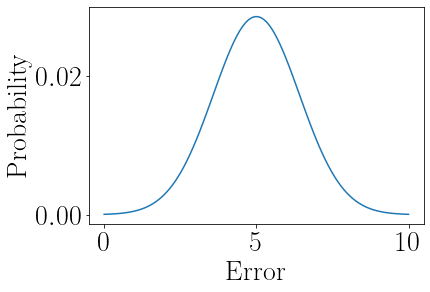
\includegraphics[width=\linewidth]{./img/distributions/normal.png}
    \caption{Gaussian}
    \vspace{4ex}
    \label{n_5_2_hist}
  \end{minipage}%%
  \begin{minipage}[b]{0.5\linewidth}
    \centering
    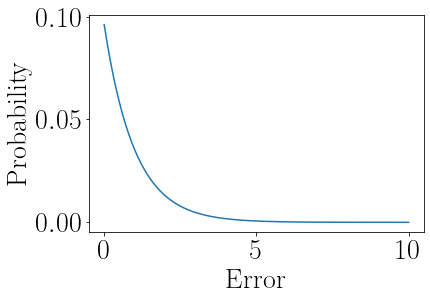
\includegraphics[width=\linewidth]{./img/distributions/exponential.png}
    \caption{Exponential}
    \vspace{4ex}
  \end{minipage}
  \begin{minipage}[b]{0.5\linewidth}
    \centering
    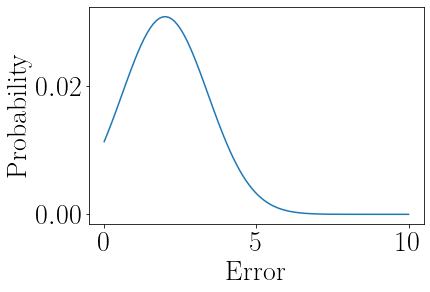
\includegraphics[width=\linewidth]{./img/distributions/normal_n_2_2.png}
    \caption{Normal N(2,2)}
    \vspace{4ex}
    \label{n_2_2_hist}
  \end{minipage}%% 
  \begin{minipage}[b]{0.5\linewidth}
    \centering
    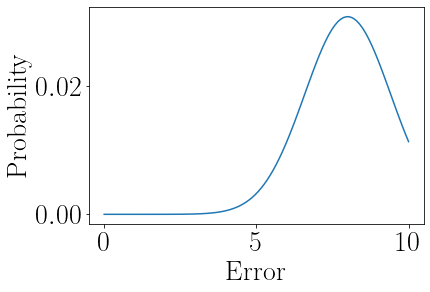
\includegraphics[width=\linewidth]{./img/distributions/normal_n_8_2.png}
    \caption{Normal N(8,2)}
    \vspace{4ex}
  \end{minipage}
  \begin{minipage}[b]{0.5\linewidth}
    \centering
    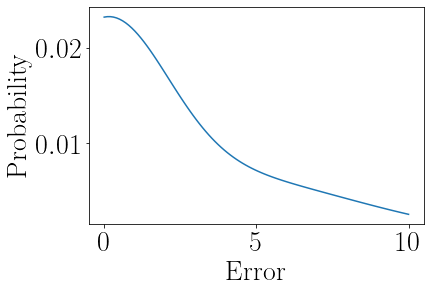
\includegraphics[width=\linewidth]{./img/distributions/heavy_tailed_2.png}
    \caption{Heavy Tailed}
    \vspace{4ex}
    \label{heavy_tailed_distributions}
  \end{minipage}%% 
  \begin{minipage}[b]{0.5\linewidth}
    \centering
    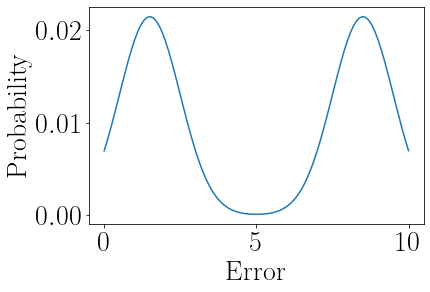
\includegraphics[width=\linewidth]{./img/distributions/twin_peaks.png}
    \caption{Bimodal}
    \label{bimodal_distribution}
    \vspace{4ex}
  \end{minipage}
  \caption{Six possible error metric distributions.}
  \label{fig:error_metric_distributions}
\end{figure}
\begin{figure}[ht]
  \begin{minipage}[b]{0.5\linewidth}
    \centering
    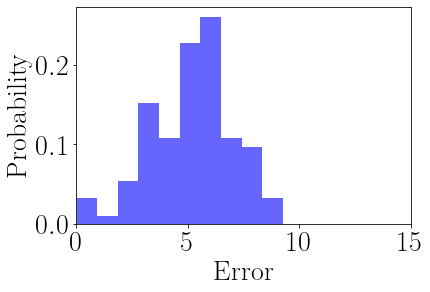
\includegraphics[width=\linewidth]{./img/distributions/normal_hist.png}
    \caption{Normal N(5,2)}
    \vspace{4ex}
  \end{minipage}%%
  \begin{minipage}[b]{0.5\linewidth}
    \centering
    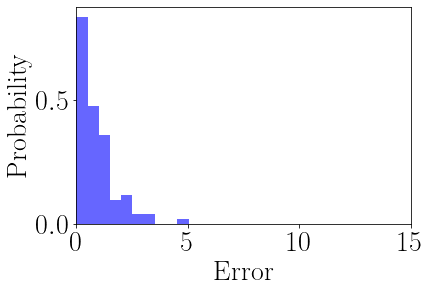
\includegraphics[width=\linewidth]{./img/distributions/exponential_hist.png}
    \caption{Exponential}
    \vspace{4ex}
    \label{exponential_hist}
  \end{minipage}
  \begin{minipage}[b]{0.5\linewidth}
    \centering
    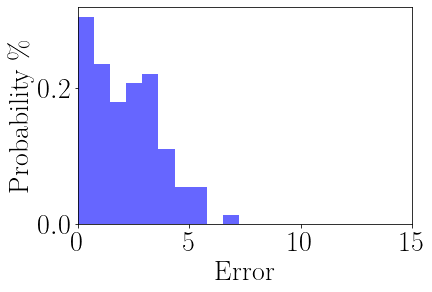
\includegraphics[width=\linewidth]{./img/distributions/normal_n_2_2_hist.png}
    \caption{Normal N(2,2)}
    \vspace{4ex}
  \end{minipage}%% 
  \begin{minipage}[b]{0.5\linewidth}
    \centering
    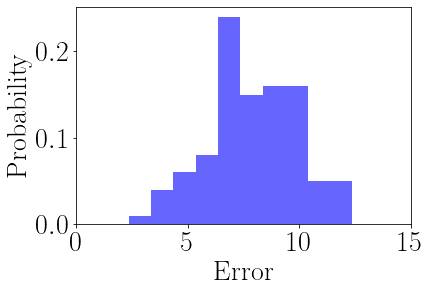
\includegraphics[width=\linewidth]{./img/distributions/normal_n_8_2_hist.png}
    \caption{Normal N(8,2)}
    \vspace{4ex}
  \end{minipage}
  \begin{minipage}[b]{0.5\linewidth}
    \centering
    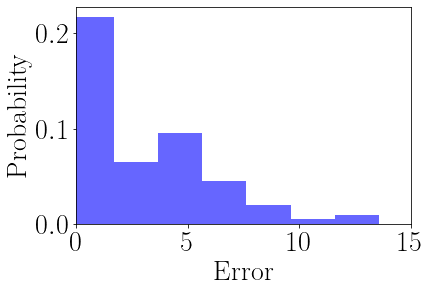
\includegraphics[width=\linewidth]{./img/distributions/heavy_tailed_2_hist.png}
    \caption{Heavy Tailed}
    \vspace{4ex}
    \label{heavy_tailed_distributions_hist}
  \end{minipage}%% 
  \begin{minipage}[b]{0.5\linewidth}
    \centering
    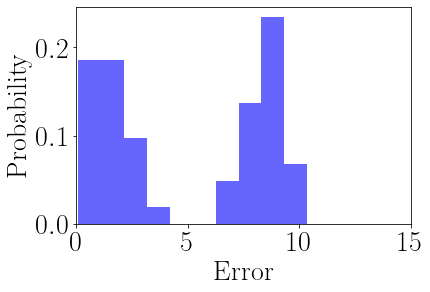
\includegraphics[width=\linewidth]{./img/distributions/twin_peaks_hist.png}
    \caption{Bimodal}
    \label{bimodal_distribution_hist}
    \vspace{4ex}
  \end{minipage}
  \caption{Six histograms from 100 samples of possible error metric distributions.}
  \label{fig:error_metric_distributions_hist}
\end{figure}
% \begin{figure}[htb]
%   \centering
%   \minipage{0.40\textwidth}
%   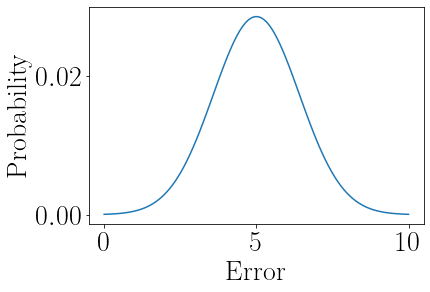
\includegraphics[width=\linewidth]{./img/distributions/normal.png}
%   \caption{Gaussian}
%   \endminipage

%   \minipage{0.40\textwidth}
%   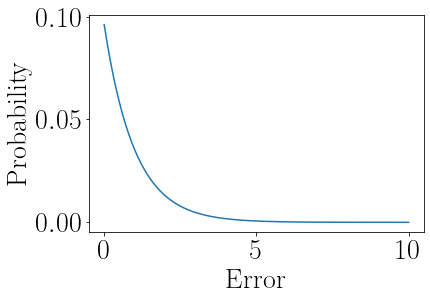
\includegraphics[width=\linewidth]{./img/distributions/exponential.png}
%   \caption{Exponential}
%   \endminipage
%   \\
%   \minipage{0.40\textwidth}
%   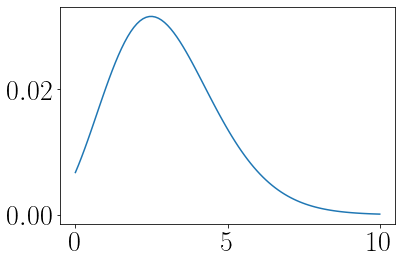
\includegraphics[width=\linewidth]{./img/distributions/poisson.png}
%   \caption{Poisson}
%   \endminipage

%   \minipage{0.48\textwidth}
%   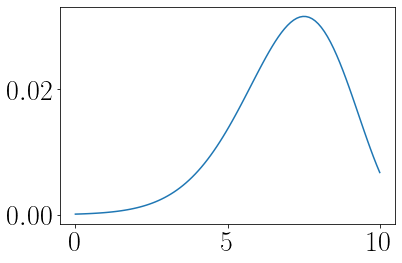
\includegraphics[width=\linewidth]{./img/distributions/reverse_poisson.png}
%   \caption{Reverse Poisson}
%   \endminipage
%   \caption{Different possible distributions of error metrics, which one is best?}
% \end{figure}